\section{The timing artefact}\label{sec:timing}

Renewal fees are due from grant, not from filing. If two otherwise identical patents are filed on the same day and
one is granted two years earlier, by ten years from filing its owner has faced two more renewal decisions, and it
is more likely to have lapsed for that reason alone. Comparisons of survival from filing therefore mix value with
exposure whenever grant speeds differ between the groups being compared.

They differ sharply between domestic and foreign owners in China and Korea. For small owners, the median grant lag
is 3.5~years for domestic and 5.5~years for foreign patents in China, and 2.4 against 5.0~years in Korea; many
foreign applications enter through the PCT national phase, which adds time before examination starts. In the
rich-economy offices the domestic--foreign difference is about one year or less.

Table~\ref{tab:timing} and Figure~\ref{fig:timing} show the consequence. Measured as survival to ten years from
filing, with citation controls, small domestic firms in the emerging-market offices appear 8.4~points behind their
rich-economy counterparts, and universities 30~points behind. Adding X/Y citations or citations by age four changes
these figures by less than one point. Adding the grant lag closes most of the gap, and measuring survival from grant
reverses it for firms: by eight years after grant, emerging-market firms of every size are \emph{ahead} of
rich-economy firms relative to foreign owners in the same office. Only the university gap survives, at a third of
its original size.

\begin{table}[ht]
\centering
\begin{threeparttable}
\caption{The emerging-market gap, measured from filing and from grant}\label{tab:timing}
\small
% Source: em-patent-value notes sections 4 and 9 (09_heterogeneity.py, 16_rich_quality.py, 16c_survival_from_grant.py)
\begin{tabular}{lS[table-format=-2.1]S[table-format=-2.1]S[table-format=-2.1]}
\toprule
 & \multicolumn{2}{c}{Alive 10 years from filing} & {Alive 8 years} \\
\cmidrule(lr){2-3}
Owner group & {Citations} & {+ grant lag} & {from grant} \\
\midrule
Firms, 1--9 families     & -8.4  & 0.3   & 3.5 \\
Firms, 10--99            & -3.6  & {}    & 9.4 \\
Firms, 100--999          & -0.3  & 5.8   & 11.6 \\
Firms, 1{,}000+          & -2.4  & {}    & 6.2 \\
Universities             & -29.8 & -9.7  & -11.8 \\
\bottomrule
\end{tabular}
\begin{tablenotes}\footnotesize
\item Notes: Extra domestic--foreign gap in survival in the emerging-market offices (China, Korea, Brazil) relative to
the rich-economy offices, in percentage points. Linear probability models with office $\times$ year, office $\times$
field and office $\times$ owner-group fixed effects and office-specific citation slopes; owner groups estimated
jointly in the full sample. Standard errors (clustered by owner) are 0.5--3.5 points; see Appendix. Blank: not
estimated in that specification.
\end{tablenotes}
\end{threeparttable}
\end{table}

\begin{figure}[ht]
\centering
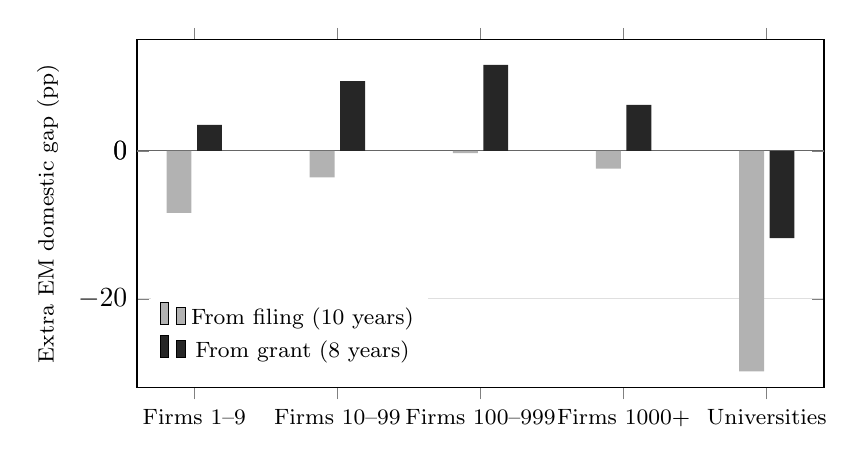
\begin{tikzpicture}
\begin{axis}[
  ybar, bar width=9pt, width=0.85\textwidth, height=6cm,
  symbolic x coords={Firms 1--9, Firms 10--99, Firms 100--999, Firms 1000+, Universities},
  xtick=data, x tick label style={font=\footnotesize, align=center},
  ylabel={Extra EM domestic gap (pp)}, ylabel style={font=\footnotesize},
  ymin=-32, ymax=15, ymajorgrids, grid style={gray!25},
  legend style={font=\footnotesize, at={(0.02,0.04)}, anchor=south west, draw=none},
  extra y ticks={0}, extra y tick style={grid=major, grid style={black!60}},
]
\addplot[fill=gray!60, draw=none] coordinates
  {(Firms 1--9,-8.4) (Firms 10--99,-3.6) (Firms 100--999,-0.3) (Firms 1000+,-2.4) (Universities,-29.8)};
\addplot[fill=black!85, draw=none] coordinates
  {(Firms 1--9,3.5) (Firms 10--99,9.4) (Firms 100--999,11.6) (Firms 1000+,6.2) (Universities,-11.8)};
\legend{From filing (10 years), From grant (8 years)}
\end{axis}
\end{tikzpicture}
\caption{Measured from grant, the emerging-market gap disappears for firms. Same estimates as
Table~\ref{tab:timing}.}\label{fig:timing}
\end{figure}

The lesson is general. Grant speeds differ across offices, owner nationalities, entry routes and periods, so any
comparison of patent survival or renewal-based value should start the clock at grant, or at the first renewal fee.
